
\documentclass[11pt,a4paper]{article}
\usepackage[margin=1.8cm]{geometry}
\usepackage{amsmath,amssymb}
\usepackage{tikz}
\usepackage{xcolor}
\usepackage{parskip}
\usepackage[T1]{fontenc}
\usepackage[utf8]{inputenc}
\usepackage[dutch]{babel}
\usepackage{newtxtext,newtxmath}
\usetikzlibrary{arrows.meta,calc,positioning}

\setlength{\parskip}{0.6em}
\setlength{\parindent}{0pt}

\newcommand{\uncertain}[1]{\textit{\textcolor{gray}{#1}}}

\newcommand{\atombase}[1]{
\begin{tikzpicture}[scale=0.78]
    \fill[red!65] (0,0) circle (0.8);
    \draw[green!60!black, line width=2.2pt] (0,0) circle (1.0);
    \draw[blue, line width=1.5pt] (0,0) circle (2.15);
    #1
\end{tikzpicture}
}

\title{Notebook 2012 --- Pagina's 27--31}
\author{}
\date{}

\begin{document}
\maketitle

\uncertain{Pagina 26 is op verzoek overgeslagen. De reconstructie hieronder volgt de handgeschreven notities zo letterlijk mogelijk. Waar een symbool of label niet volledig scherp leesbaar is, is de meest waarschijnlijke lezing gekozen.}

\clearpage
\section*{Pagina 27}

\begin{minipage}[t]{0.48\textwidth}
\subsection*{Linkerhelft}
\begin{align*}
a_0 &= \frac{\hbar}{m_e c \alpha} \\
    &= 0{,}52917721092 \cdot 10^{-10}\ \text{meter}
\end{align*}

\uncertain{Groene notitie: ``Wat is $\alpha$''; daarnaast vermoedelijk $\alpha \approx \frac{1}{137}$.}

\atombase{
    \fill[blue] (2.15,0.05) circle (0.09);
    \draw[densely dotted,->] (0,0) -- (2.02,0.05);
    \node[right] at (2.2,0.05) {$m_e c$};
    \node[right] at (1.45,-1.95) {$N_1=a_0$};
}

\[
\frac{1.054571726 \cdot 10^{-34}}
     {9.10938291 \cdot 10^{-31} \cdot 299792458 \cdot 0.00729735256}
\]
\end{minipage}
\hfill
\begin{minipage}[t]{0.48\textwidth}
\subsection*{Rechterhelft}
\begin{align*}
h &= 4\pi m_e v_e a_0 \\
  &= 6{,}62606957 \cdot 10^{-34}\ \text{J\,s}
\end{align*}

\atombase{
    \fill[blue] (1.9,1.0) circle (0.1);
    \node[right] at (2.02,1.15) {$4\pi$};
    \node[right] at (2.08,0.82) {$m_e v_e$};
    \node[right] at (1.45,-1.95) {$N_1=a_0$};
}

\[
4\pi \cdot 9.10938291 \cdot 10^{-31}
\cdot 1.0938456336 \cdot 10^{6}
\cdot 0.52917721092 \cdot 10^{-10}
\]
\end{minipage}

\clearpage
\section*{Pagina 28}

\begin{minipage}[t]{0.48\textwidth}
\subsection*{Linkerhelft}
\begin{align*}
h &= \frac{4\pi F_{\max} R_c^2}{v_e} \\
  &= 6{,}62606957 \cdot 10^{-34}\ \text{J\,s}
\end{align*}

\uncertain{Losse notitie rechtsboven: ``Planck is impuls/hoekmoment'' (gedeeltelijk onzeker).}

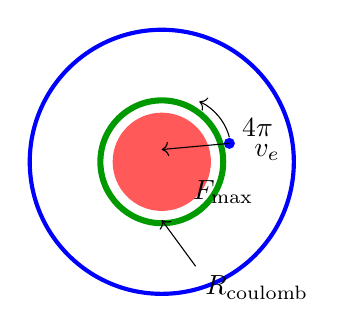
\begin{tikzpicture}[scale=0.78]
    \fill[red!65] (0,0) circle (0.8);
    \draw[green!60!black, line width=2.2pt] (0,0) circle (1.0);
    \draw[blue, line width=1.5pt] (0,0) circle (2.15);
    \fill[blue] (1.1,0.3) circle (0.09);
    \draw[->] (1.1,0.4) arc[start angle=15,end angle=65,radius=0.9];
    \draw[->] (1.1,0.3) -- (0.0,0.2);
    \node[right] at (1.15,0.55) {$4\pi$};
    \node[right] at (1.35,0.15) {$v_e$};
    \node[below] at (1.0,-0.15) {$F_{\max}$};
    \draw[->] (0.55,-1.7) -- (0.0,-0.95);
    \node[below right] at (0.55,-1.7) {$R_{\text{coulomb}}$};
\end{tikzpicture}

\[
\frac{4\pi \cdot 29.053507333 \cdot (1.46097017 \cdot 10^{-15})^2}
     {1.0938456336 \cdot 10^{6}}
\]
\end{minipage}
\hfill
\begin{minipage}[t]{0.48\textwidth}
\subsection*{Rechterhelft}
\begin{align*}
a_0 &= \frac{h}{4\pi m_e v_e} \\
    &= 0{,}52917721 \cdot 10^{-10}
\end{align*}

\atombase{
    \draw[densely dotted,->] (0,0) -- (2.0,0.0);
    \node[right] at (1.45,-1.95) {$N_1=a_0$};
}

\[
\frac{6.62606957 \cdot 10^{-34}}
     {4\pi \cdot 9.10938291 \cdot 10^{-31} \cdot 1.0938456336 \cdot 10^{6}}
\]
\end{minipage}

\clearpage
\section*{Pagina 29}

\begin{minipage}[t]{0.48\textwidth}
\subsection*{Linkerhelft}
\begin{align*}
a_0 &= \frac{c^2 R_c}{2 C_e} \\
    &= 0{,}52917721092 \cdot 10^{-10}
\end{align*}

\begin{align*}
\lambda &= \frac{2 C_e}{c}
\end{align*}

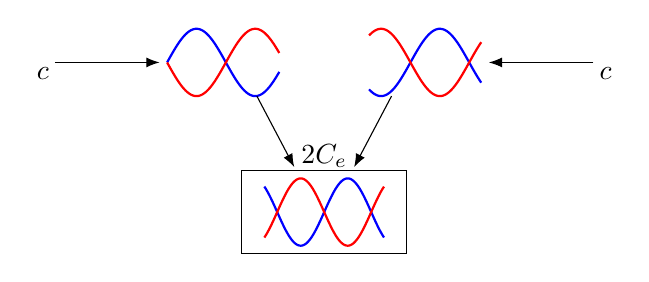
\begin{tikzpicture}[scale=0.95,>=Latex]
    % left incoming packet
    \draw[->] (-3.6,0) -- (-2.2,0);
    \node[left] at (-3.55,-0.15) {$c$};
    \draw[blue,thick,domain=-2.1:-0.6,samples=80] plot (\x,{0.45*sin(deg(4*(\x+2.1)))});
    \draw[red,thick,domain=-2.1:-0.6,samples=80] plot (\x,{-0.45*sin(deg(4*(\x+2.1)))});
    % right incoming packet
    \draw[->] (3.6,0) -- (2.2,0);
    \node[right] at (3.55,-0.15) {$c$};
    \draw[blue,thick,domain=0.6:2.1,samples=80] plot (\x,{0.45*sin(deg(4*(\x-0.6)+180))});
    \draw[red,thick,domain=0.6:2.1,samples=80] plot (\x,{-0.45*sin(deg(4*(\x-0.6)+180))});
    % arrows to overlap
    \draw[->] (-0.9,-0.45) -- (-0.4,-1.4);
    \draw[->] (0.9,-0.45) -- (0.4,-1.4);
    % overlap box
    \draw (-1.1,-2.55) rectangle (1.1,-1.45);
    \node at (0.0,-1.25) {$2 C_e$};
    \draw[blue,thick,domain=-0.8:0.8,samples=80] plot (\x,{-2.0+0.45*sin(deg(5*\x))});
    \draw[red,thick,domain=-0.8:0.8,samples=80] plot (\x,{-2.0-0.45*sin(deg(5*\x))});
\end{tikzpicture}

\uncertain{De doorgestreepte notitie onderaan is te onduidelijk om betrouwbaar over te nemen.}
\end{minipage}
\hfill
\begin{minipage}[t]{0.48\textwidth}
\subsection*{Rechterhelft}
\begin{align*}
R_c &= \frac{c^2}{a_0\, 2 C_e} \\
    &= 1{,}46097017 \cdot 10^{-15}
\end{align*}

\[
\frac{299792458^2}
     {0.52917721092 \cdot 10^{-10} \cdot 2 \cdot 1.0938456336 \cdot 10^{6}}
\]

\uncertain{Deze paginahelft bevat verder vrijwel alleen de numerieke invulling.}
\end{minipage}

\clearpage
\section*{Pagina 30}

\begin{minipage}[t]{0.48\textwidth}
\subsection*{Linkerhelft}
\begin{align*}
a_0 &= h \cdot \frac{c^2}{8\pi F_{\max} v_e R_c} \\
    &= 0{,}529177211 \cdot 10^{-10}
\end{align*}

\[
6.62606957 \cdot 10^{-34}
\cdot
\frac{299792458^2}
     {8\pi \cdot 29.053507333 \cdot 1.0938456336 \cdot 10^{6}
      \cdot 1.46097017 \cdot 10^{-15}}
\]
\end{minipage}
\hfill
\begin{minipage}[t]{0.48\textwidth}
\subsection*{Rechterhelft}
\begin{align*}
a_0 &= \frac{F_{\max} R_c}{m_e v_e^2}
\end{align*}

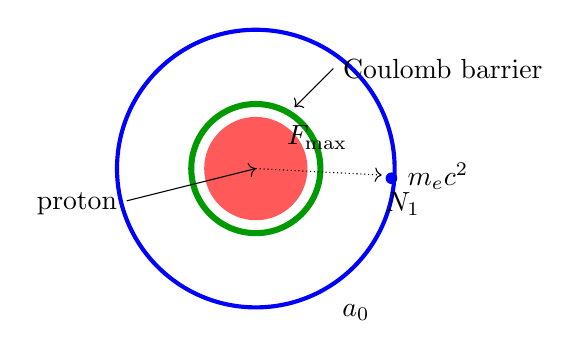
\begin{tikzpicture}[scale=0.82]
    \fill[red!65] (0,0) circle (0.8);
    \draw[green!60!black, line width=2.2pt] (0,0) circle (1.0);
    \draw[blue, line width=1.5pt] (0,0) circle (2.15);
    \fill[blue] (2.1,-0.15) circle (0.09);
    \draw[->] (-2.0,-0.5) -- (0.0,0.0);
    \node[left] at (-2.0,-0.55) {proton};
    \draw[densely dotted,->] (0,0) -- (1.95,-0.1);
    \node[above] at (0.95,0.15) {$F_{\max}$};
    \node[right] at (2.2,-0.12) {$m_e c^2$};
    \node[below] at (1.55,-1.95) {$a_0$};
    \node[right] at (1.85,-0.55) {$N_1$};
    \draw[->] (1.2,1.55) -- (0.6,0.95);
    \node[right] at (1.2,1.55) {Coulomb barrier};
\end{tikzpicture}

\[
\frac{29.053507333 \cdot (1.46097017 \cdot 10^{-15})^2}
     {9.10938291 \cdot 10^{-31} \cdot (1.0938456336 \cdot 10^{6})^2}
\]
\end{minipage}

\clearpage
\section*{Pagina 31}

\begin{minipage}[t]{0.48\textwidth}
\subsection*{Linkerhelft}
\begin{align*}
m_e &= \frac{2 F_{\max} R_c}{c^2} \\
    &= 9{,}10938287 \cdot 10^{-31}
\end{align*}

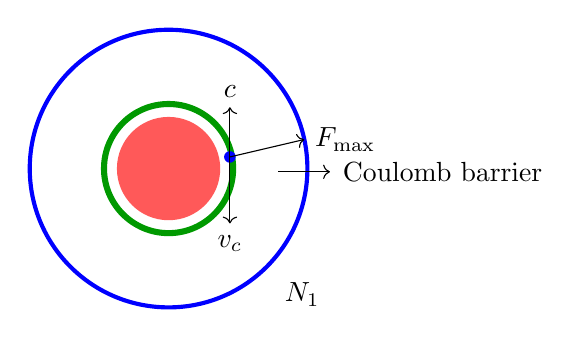
\begin{tikzpicture}[scale=0.82]
    \fill[red!65] (0,0) circle (0.8);
    \draw[green!60!black, line width=2.2pt] (0,0) circle (1.0);
    \draw[blue, line width=1.5pt] (0,0) circle (2.15);
    \fill[blue] (0.95,0.18) circle (0.09);
    \draw[->] (0.95,0.18) -- (2.1,0.45);
    \node[right] at (2.12,0.45) {$F_{\max}$};
    \draw[->] (0.95,0.18) -- (0.95,0.95);
    \node[above] at (0.95,0.95) {$c$};
    \draw[->] (0.95,0.18) -- (0.95,-0.85);
    \node[below] at (0.95,-0.88) {$v_c$};
    \draw[->] (1.7,-0.05) -- (2.5,-0.05);
    \node[right] at (2.55,-0.05) {Coulomb barrier};
    \node[right] at (1.65,-1.95) {$N_1$};
\end{tikzpicture}

\[
\frac{2 \cdot 29.053507333 \cdot 1.46097017 \cdot 10^{-15}}
     {299792458^2}
\]
\end{minipage}
\hfill
\begin{minipage}[t]{0.48\textwidth}
\subsection*{Rechterhelft}
\begin{align*}
v_e &= \left(\frac{R_c}{\pi}\right)
       \sqrt{\frac{F_{\max}}{2 R_{\text{proton}} m_{\text{proton}}}} \\
    &= 1{,}0938456336 \cdot 10^{6}
\end{align*}

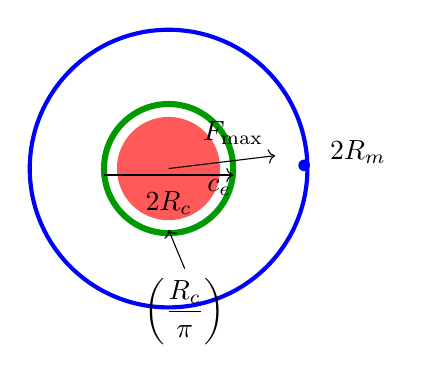
\begin{tikzpicture}[scale=0.82]
    \fill[red!65] (0,0) circle (0.8);
    \draw[green!60!black, line width=2.2pt] (0,0) circle (1.0);
    \draw[blue, line width=1.5pt] (0,0) circle (2.15);
    \fill[blue] (2.1,0.05) circle (0.09);
    \node[right] at (2.35,0.25) {$2R_m$};
    \draw[->] (-1.0,-0.1) -- (1.0,-0.1);
    \node[below] at (0,-0.2) {$2R_c$};
    \draw[->] (0,0) -- (1.65,0.2);
    \node[above] at (1.0,0.22) {$F_{\max}$};
    \node[below right] at (0.45,-0.02) {$c_e$};
    \draw[->] (0.25,-1.55) -- (0,-0.95);
    \node[below] at (0.25,-1.55) {$\left(\dfrac{R_c}{\pi}\right)$};
\end{tikzpicture}

\[
\left(\frac{1.46097017 \cdot 10^{-15}}{\pi}\right)
\sqrt{
\frac{29.053507333}
     {2 \cdot 1.4600300097 \cdot 10^{-15}
      \cdot 1.672621777 \cdot 10^{-27}}
}
\]
\end{minipage}

\end{document}
